\documentclass{article}
\usepackage{booktabs}
\usepackage{amsthm, amssymb, amsmath}
\usepackage{mathtools}
\usepackage{graphicx}
\usepackage{algorithm}
\usepackage{algorithmic}

\usepackage{todonotes}

\usepackage{stmaryrd, color, tikz, dsfont}
\usepackage{booktabs}

\DeclareMathOperator*{\argmax}{arg\,max}
\DeclareMathOperator*{\argmin}{arg\,min}

\newcommand{\dbn}{{\sc dbn}}
\newcommand{\dbns}{{\sc dbn}s}
\newcommand{\bn}{{\sc bn}}
\newcommand{\bdn}{{\sc bdn}}
\newcommand{\Pa}{\mathit{Pa}}
\renewcommand{\dag}{{\sc dag}}
\newcommand{\holderFig}[1]{\missingfigure[figwidth=\linewidth, figheight=6cm]{{#1}}}
\newcommand{\ra}[1]{\renewcommand{\arraystretch}{#1}}


\newtheorem{theorem}{Theorem}
\newtheorem{lemma}{Lemma}

% Recommended, but optional, packages for figures and better typesetting:
\usepackage{microtype}
\usepackage{subcaption}

% hyperref makes hyperlinks in the resulting PDF.
% If your build breaks (sometimes temporarily if a hyperlink spans a page)
% please comment out the following usepackage line and replace
% \usepackage{icml2018} with \usepackage[nohyperref]{icml2018} above.
\usepackage{hyperref}

% Attempt to make hyperref and algorithmic work together better:
\newcommand{\theHalgorithm}{\arabic{algorithm}}

% Use the following line for the initial blind version submitted for review:
\usepackage{icml2019}

\usepackage{xr}
\externaldocument{dnPaper}

\begin{document}
	\title{Technical Supplement}
	\date{}
	\maketitle
	
	\section{Proof of Lemmas and Theorems}
		\begin{lemma}
%			\label{thm:action-awareness}
			Consider a \bdn{} where an $\epsilon$-greedy agent has awareness $\mathcal{X}^t \subseteq \mathcal{X}^+, A^t \subset A^+$, and an expert acts with respect to (\ref{eqn:last-spoken-interval}-\ref{eqn:better-action-utterance}). As $k \rightarrow \infty$, either $PE(\pi_{t+k}) \rightarrow c$ with $c \leq \beta$ or the expert utters (\ref{eqn:better-action-utterance}) such that $\mathcal{A}' \neq \emptyset$.
		\end{lemma}
		\begin{proof}
			For finite $\mu$, $(t+k) - t' > \mu$ as $k \rightarrow \infty$, satisfying (\ref{eqn:last-spoken-interval}). 
			
			Given $\mathcal{A}^t$ remains fixed, the agent's policy will eventually converge to some policy $\pi$. If $PE(\pi) < \beta$, we are done. If $PE(\pi) \geq \beta$, then (\ref{eqn:suboptimal-performance}) will be satisfied.
			
			Since the agent is $\epsilon$-greedy, at every time step it has a non-zero probability of performing all actions $a \in v(\mathcal{A}_t)$, meaning that eventually $\mathcal{A}^e = \mathcal{A}^t$. Further, since $\pi \neq \pi_+$, there must exist some $b \in v(\mathcal{B}^+)$ and $a' \in v(\mathcal{A}^+)$ such that $\forall a \in \mathcal{A}^t, EU(a' | b) > EU(a | b)$, thereby satisfying (\ref{eqn:better-action-available}).
			
			Since the agent is $\epsilon$-greedy, it is guaranteed to eventually perform $a^* = \argmax_{a \in v(\mathcal{A}^t)} EU(a | b)$ in in state $b$, thus making (\ref{eqn:minimal-action}) true for a non-empty value of $\mathcal{A}'$.
			
			(\ref{eqn:last-spoken-interval}-\ref{eqn:minimal-action}) are not mutually exclusive, so all four will eventually be true at once, causing the expert to utter (\ref{eqn:better-action-utterance}) for non-empty $\mathcal{A}'$.
		\end{proof}

		\begin{lemma}
%			\label{theorem:state-space-awareness}
			Consider an agent with awareness $\mathcal{X}^t \subset \mathcal{X}^+$, $\mathcal{A}^t = \mathcal{A}^+$. If $\exists b', \exists b \neq b', b[\mathcal{B}^t] = b'[\mathcal{B}^t]$ and $\pi_+(b) \neq \pi_+(b')$, then as $k \rightarrow \infty$, either $PE(\pi_{t+k}) \rightarrow c \leq \beta$, or the expert utters (\ref{eqn:misunderstanding-a-anc}) such that $B' \notin \mathcal{B}^t$
		\end{lemma}
		
		\begin{proof}
			If the agent converges to some policy $\pi$ such that $PE(\pi) \leq \beta$, we are done.
			
			Assume $a = \pi_+(b)$ and $a' = \pi_+(b')$. Consider that for all $k$, $P(b_{t+k} = b) > 0$, and (since the agent is $\epsilon$-greedy) $P(\pi_{t+k}(b) = a') > 0$, where $a' = \pi_+(b')$. 
			
			If $PE(\pi) \geq$, then at some time $t + k_1$ where $(t + k_1) - t' > \mu$ and $b_{t + k_1} = b$ the agent will perform $a'$, thus satisfying (\ref{eqn:last-spoken-interval}-\ref{eqn:minimal-action}) and causing the expert to utter $EU(a | w^b_{t + k_1}) > EU(a' | w^b_{t + k_1})$.
			
			By similar reasoning, at some time $b_{t + k_2} = b'$ the expert will utter $EU(a', w^b_{t + k_2}) > EU(a, w^b_{t + k_2})$.
			
			Under $\mathcal{B}^t$, $\llbracket w^s_{t + k_1} \rrbracket = \llbracket w^s_{t + k_2} \rrbracket$, so the agent will ask (\ref{eqn:misunderstanding-q}) with answer $B \notin \mathcal{B}^t$.
		\end{proof}
		
		\begin{lemma}
%			\label{thm:reward-scope-awareness}
			Consider an $\epsilon$-greedy agent with awareness $\mathcal{A}^t = \mathcal{A}^+$, $scope_t(\mathcal{R}) \subseteq scope_+(\mathcal{R})$. As $k \rightarrow \infty$, there exists a $K$ such that $\forall s, \forall k \geq K$, $\mathcal{R}_{t+k}(s) = \mathcal{R}_{+}(s)$.
		\end{lemma}
		\begin{proof}
			Since the $\mathcal{A}^t = \mathcal{A}^+$, and is $\epsilon$-greedy, then over infinite time the agent will eventually enter $s$ at some time $i$, receiving reward $\mathcal{R}_+(s)$, and update its current reward function so that $\mathcal{R}_{i}(s) = \mathcal{R}_+(s)$. If the agent has previously encountered another $s'$ such that $s[scope_t(\mathcal{R})] = s'[scope_t(\mathcal{R})]$ and $\mathcal{R}_+(s) \neq \mathcal{R}_+(s')$, the partial descriptions (\ref{eqn:trial-monotonic}) for $s$ and $s'$ will conflict. The agent resolves this by asking (\ref{eqn:unforeseen-reward-q}), receiving an answer differentiating $s$ from $s'$ in $\mathcal{R}_+$. 
		\end{proof}
		
	\begin{theorem}
%		\label{thm:full-unawareness-guarantee}
		Consider an agent with initial awareness $\mathcal{X}^0 \subseteq \mathcal{X}^+, A^0 \subseteq A^+ ,scope_0(\mathcal{R}) \subseteq scope_+(\mathcal{R})$ following algorithm \ref{alg:full-system} (with $\kappa = 0$). As $t \rightarrow \infty$, $PE(\pi_{t}) \rightarrow c \leq \beta$.
	\end{theorem}
	\begin{proof}
		By repeatedly applying theorems \ref{thm:action-awareness}-\ref{thm:reward-scope-awareness}, either $PE(\pi_t) \rightarrow c \leq$ (in which case we are done), or there exists a $K$ where $\mathcal{A}^K = \mathcal{A}^+$, $\mathcal{R}_K = \mathcal{R}_+$, and $\mathcal{X}^K = \mathcal{B}^k \cup \mathcal{O}^K$. Here, $\mathcal{B}^K$ contains all variables $\mathcal{B} \in \mathcal{B}^+$ such that there exist $b$, and $b'$ where $b[\mathcal{B}^+ \setminus B] = b'[\mathcal{B}^+ \setminus B]$ but $b[B] \neq b'[B]$ and $\pi_+(b) \neq \pi_+(b')$. In other words, $\langle \mathcal{X}^K, \mathcal{A}^K, \mathcal{R}^K \rangle$ define a related decision problem with an identical optimal policy and marginal probability distribution to the original problem, but for which the agent is fully aware.
		
		The BD-score is a \emph{consistent score}, which means that as $|D| \rightarrow \infty$, $\Pa^*$ contains all dependencies present in the true distribution, regardless of initial prior (assuming we have not pruned the search space, which is true in this case because $\kappa = 0$). As a result, as $t \rightarrow \infty$, then $\forall a \in v(\mathcal{A}^+)$, $\forall b \in \mathcal{B}^K$, $\forall y \in v(scope_+(\mathcal{R}))$, we have that $P(y | a, b, \Pa^*_t, \theta^*_t) \rightarrow P(y | a, b, \Pa^+, \theta^+)$.
		
		Since our agents probabilistic model converges to the true probabilistic distribution, and because $\mathcal{R}^K = \mathcal{R}^+$ and $\mathcal{A}^K = \mathcal{A}^+$, we have that $\pi^*_t \rightarrow \pi_+$ and therefore that $PE(\pi^*_t) \rightarrow 0$ 
	\end{proof}
	
	\section{Derivation of Equation (\ref{eqn:incremental-struct-score})}
	
	\textit{Note, the derivation below corrects an error from the original Buntine (1991) paper}.
	
	The proof that:
	
	\begin{equation}
	\textsc{BD}_{t}(X, \Pa_X) = \textsc{BD}_{t-1}(X, \Pa_X) \frac{N^{t}_{i|j} + \alpha_{i | j} - 1}{N^{t}_{.|j} + \alpha_{.|j} - 1}
	\tag{\ref{eqn:incremental-struct-score}}
	\end{equation}
	
	Follows from the definition of the multivariate-$\beta$ function in terms of the $\Gamma$-function, and the recursive structure of $\Gamma$:
	
	\begin{gather}
	\beta(n_1, \dots n_m) = \frac{\prod_{k = 0}^{m} \Gamma(n_k)}{\Gamma(\sum_{k = 0}^{m} n_k)} \\
	\label{eqn:gamma-recurse}
	\Gamma(x) = (x - 1) \Gamma(x - 1)
	\end{gather}
	
	From equation (\ref{eqn:fam-score}), we have:
	
	\begin{equation}
	\tag{\ref{eqn:fam-score}}
	\begin{aligned}
	&\textsc{BD}_t(X, Pa_X) =\\
	&\quad P(\Pa_X) \prod_{\mathclap{j \in v(\Pa_X)}} \frac{\beta(N^t_{0|j} + \alpha_{0|j}, \dots , N^t_{m | j} + \alpha_{m | j})}{\beta(\alpha_{0 | j}, \dots, \alpha_{m|j})}
	\end{aligned}
	\end{equation}
	
	Lets assume that $d_t[X] = i$ and $d_t[\Pa_X] = j$. The only difference between $BD_t(X, Pa_X)$ and $BD_{t-1}(X, Pa_X)$ is between counts $N^t_{i | j}$ and $N^{t-1}_{i | j}$ (specifically, that $N^{t-1}_{i | j}  = N^{t}_{i | j} - 1$), so we can rewrite (\ref{eqn:fam-score}) as:
	
	\begin{align*}
		&\textsc{BD}_t(X, Pa_X)\\
%		&= BD_{t-1}(X, \Pa) 
%			\frac
%			{\beta(N^t_{0 | j} + \alpha_{0|j},\dots, N^t_{i | j} + \alpha_{i|j}, \dots N^t_{m | j} + \alpha_{m|j})}
%			{\beta(N^t_{0 | j} + \alpha_{0|j}, \dots N^t_{i | j} - 1 + \alpha_{i|j}, \dots N^t_{m | j} + \alpha_{m|j})}  \\
		&= BD_{t-1}(X, \Pa) 
		\frac
			{\Gamma(\sum_{k=0}^m N^{t-1}_{k|j}) \prod_{k=0}^m\Gamma(N^t_{k|j})}
			{\Gamma(\sum_{k=0}^m N^{t}_{k|j}) \prod_{k=0}^m \Gamma(N^{t-1}_{k | j})} \\
		&= \frac
		{\Gamma((\sum_{k=0}^m N^{t}_{k|j}) - 1) \Gamma(N^t_{i|j})}
		{\Gamma(\sum_{k=0}^m N^{t}_{k|j}) \Gamma(N^{t}_{i | j} - 1)} \\
	\end{align*}
	
	Then, via (\ref{eqn:gamma-recurse}), we have:
	\begin{align*}
	&\frac
	{\Gamma((\sum_{k=0}^m N^{t}_{k|j}) - 1) \Gamma(N^t_{i|j})}
	{\Gamma(\sum_{k=0}^m N^{t}_{k|j}) \Gamma(N^{t}_{i | j} - 1)} \\
	&= \frac
	{\Gamma((\sum_{k=0}^m N^{t}_{k|j}) - 1) (N^t_{i|j} - 1) \Gamma(N^t_{i|j} - 1)}
	{((\sum_{k=0}^m N^{t}_{k|j}) - 1) \Gamma((\sum_{k=0}^m N^{t}_{k|j}) - 1) \Gamma(N^{t}_{i | j} - 1)} \\
	&= \frac
	{N^t_{i|j} - 1}
	{(\sum_{k=0}^m N^{t}_{k|j}) - 1} 
	\end{align*}
	
	And therefore that:
	
	\begin{equation}
	\textsc{BD}_{t}(X, \Pa_X) = \textsc{BD}_{t-1}(X, \Pa_X) \frac{N^{t}_{i|j} + \alpha_{i | j} - 1}{N^{t}_{.|j} + \alpha_{.|j} - 1}
	\tag{\ref{eqn:incremental-struct-score}}
	\end{equation}
		
	As required.
	
		
		\begin{figure*}
			\begin{subfigure}{0.333\textwidth}
				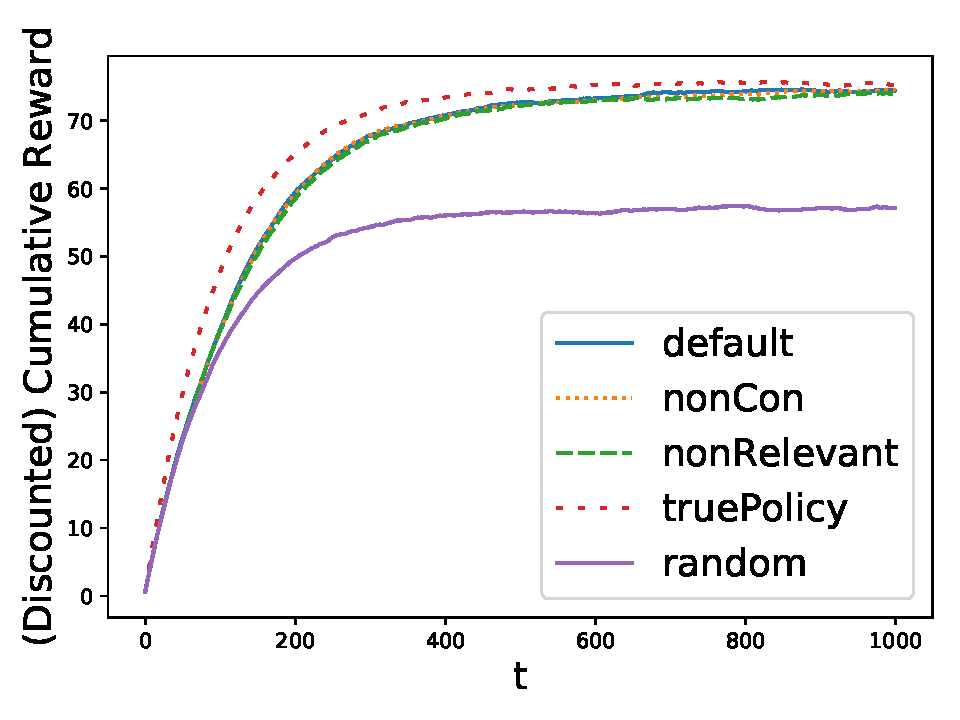
\includegraphics[width=\textwidth]{smallDNRewardsConservativity}
				\caption{}
			\end{subfigure}
			\begin{subfigure}{0.333\textwidth}
				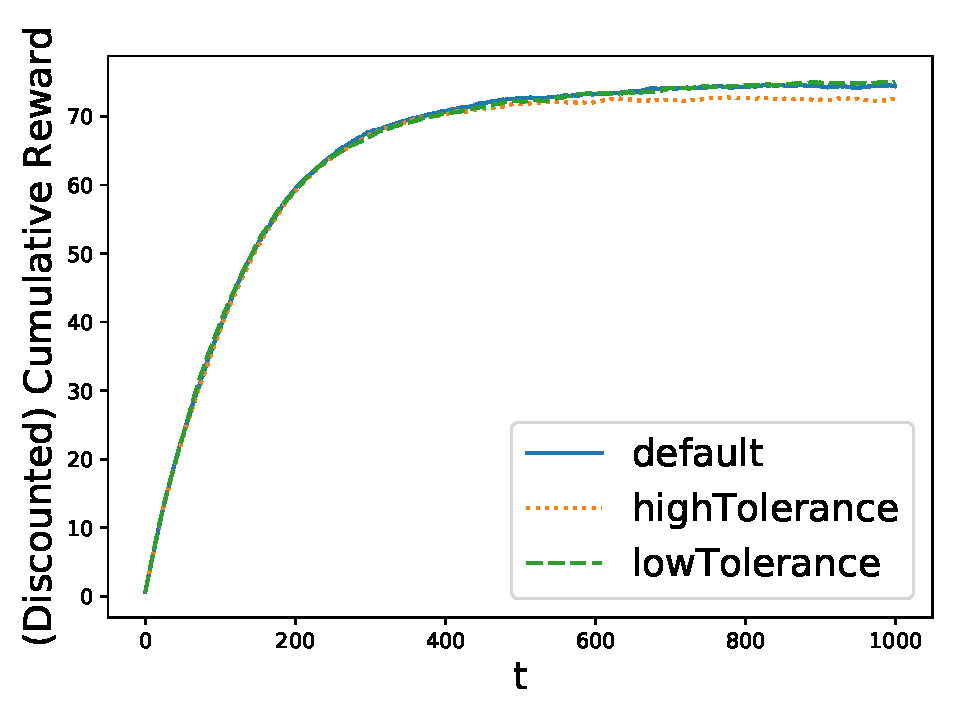
\includegraphics[width=\textwidth]{smallDNRewardsTolerance}
				\caption{}
			\end{subfigure}
			\begin{subfigure}{0.333\textwidth}
				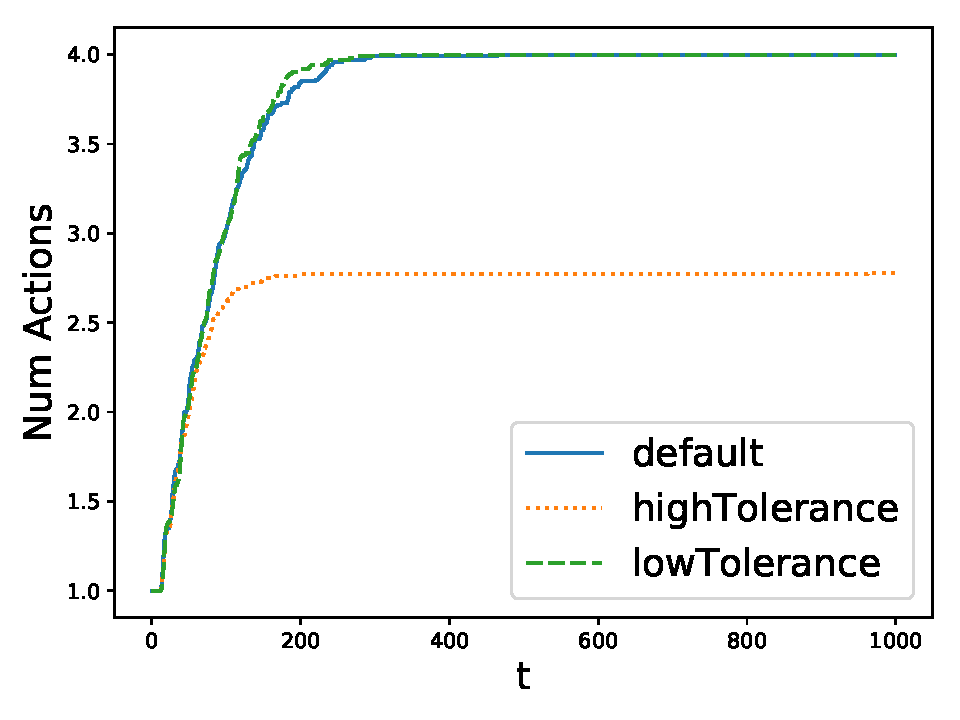
\includegraphics[width=\textwidth]{smallDNActions}
				\caption{}
			\end{subfigure}		
			\caption{Rewards and size of $|\mathcal{A}|$ over time on bdn-small.}
			\label{fig:results-small}
		\end{figure*}
		
		\begin{figure*}
			\begin{subfigure}{0.333\textwidth}
				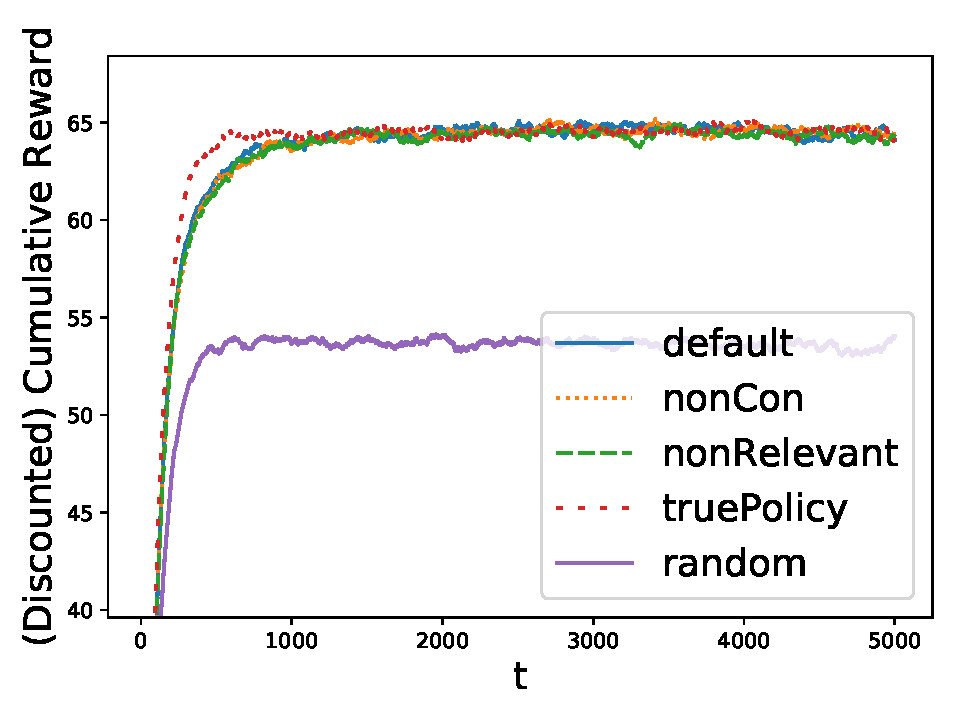
\includegraphics[width=\textwidth]{mediumDNRewardsConservativity}
				\caption{}
			\end{subfigure}
			\begin{subfigure}{0.333\textwidth}
				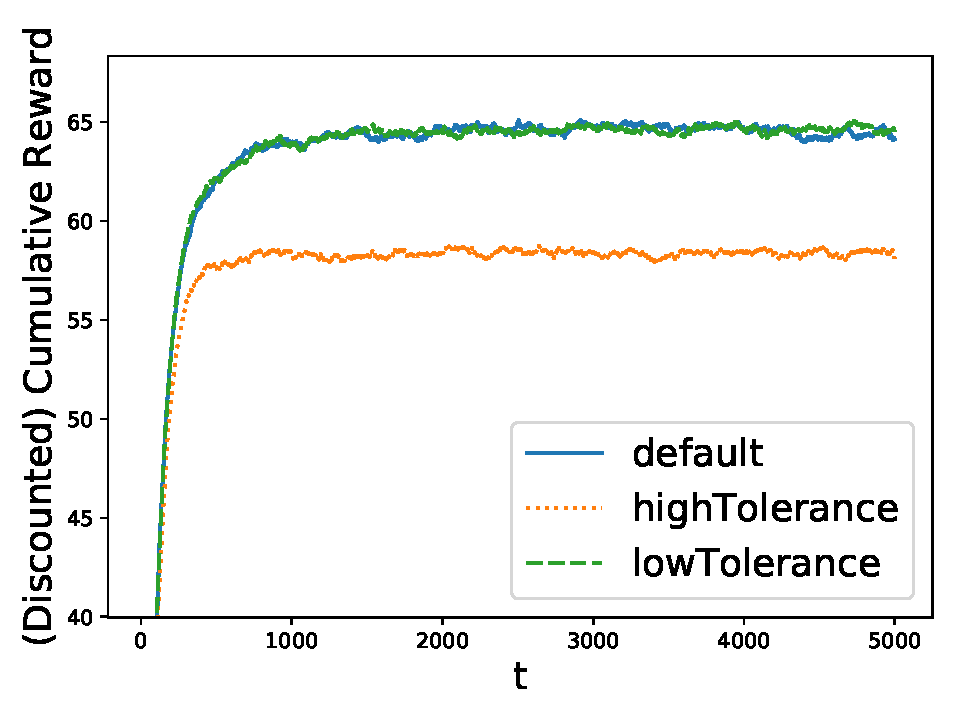
\includegraphics[width=\textwidth]{mediumDNRewardsTolerance}
				\caption{}
			\end{subfigure}
			\begin{subfigure}{0.333\textwidth}
				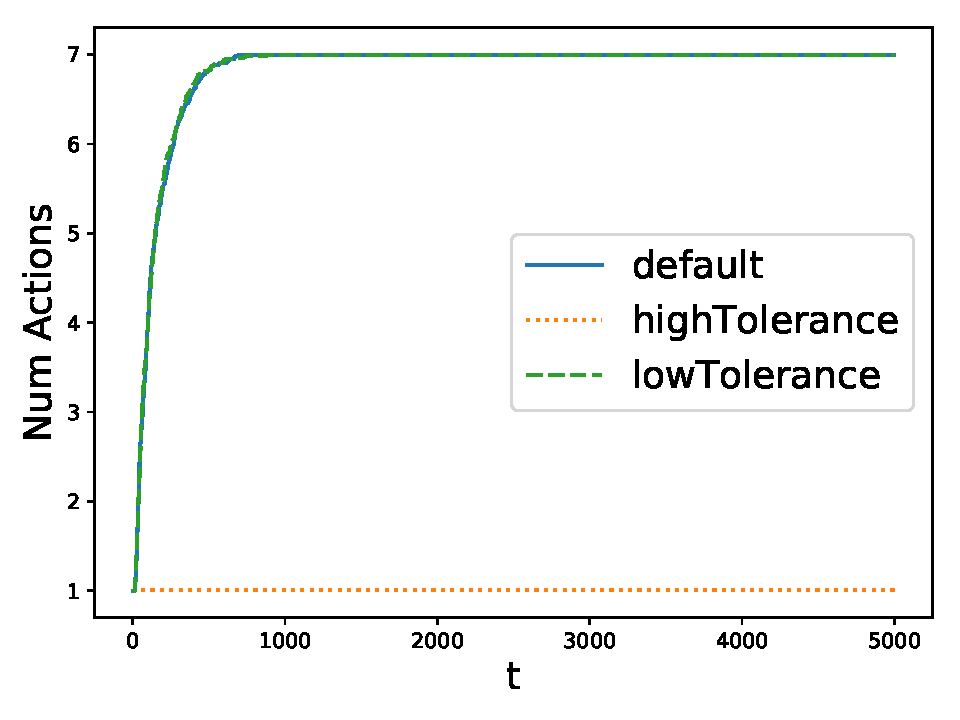
\includegraphics[width=\textwidth]{mediumDNActions}
				\caption{}
			\end{subfigure}		
			\caption{Rewards and size of $|\mathcal{A}|$ over time on bdn-medium.}
			\label{fig:results-medium}
		\end{figure*}
					
		\section{Specifications of BDNs from Experiments + Additional Results}
		
		Tables \ref{table:small}-\ref{table:large} below provide a full specification of the three randomly generated \bdn{}s used in the Experiments Section of the main paper. All variables are binary. The numbers in the $P(X|\Pa)$ give the probability of $X=1$ for each possible assignment $v(\Pa)$, where the first probability refers to the assignment of all parents to 0, and the last probability refers to the assignment of all parents to 1.
		
		Figures \ref{fig:results-small} and \ref{fig:results-medium} give the results give the results of our experiments on the small (12 variable) and medium (24 variable) \bdn{}s, using the same experimental setup as presented in Section \ref{sec:experiments} of the main paper. As with the main paper, the default agent is able to successfully converge on the true optimal policy, despite starting out unaware of factors critical to success. However, the differences in varying the expert tolerances and between the conservative and non-conservative agents are less pronounced, simply because the underlying decision problem is simpler in the smaller cases.
		
		\begin{table*}
			\centering
			\begin{tabular}{@{}lll@{}}
				X & $\Pa_X$ & $P(X | \Pa_X)$ \\
				\midrule
				B1 & $\emptyset$ & 0.50 \\
				O1 & A4 & 0.23, 0.18 \\
				B2 & $\emptyset$ & 0.84 \\
				B3 & $\emptyset$ & 0.18 \\
				O3 & A1, A3, B3 & 0.31, 0.89, 0.87, 0.15, 0.48, 0.21, 0.90, 0.06 \\
				B4 & B2 & 0.45, 0.26 \\
				O4 & A2, B1 & 0.78, 0.87, 0.12, 0.07 \\
				O2 & B2, B4, O1 & 0.04, 0.75, 0.64, 0.07, 0.36, 0.62, 0.69, 0.17 \\	
				\bottomrule
				\\
				& $scope(\mathcal{R})$ & $\mathcal{R}(s)$ \\
				\midrule
				&O4, O2, O3 & 0.98, 0.14, 0.70, 0.35, 0.38, 0.98, 0.11, 0.97
			\end{tabular}
			\caption{bdn-small: (12 Variables)}
			\label{table:small}
		\end{table*}
		
		\begin{table*}[h]
			\centering
			\begin{tabular}{@{}llp{6cm}@{}}
				X & $\Pa_X$ & $P(X | \Pa_X)$ \\
				\midrule
				B8 & $\emptyset$ & 0.05 \\
				B6 & $\emptyset$ & 0.97 \\
				B7 & $\emptyset$ & 0.01 \\
				B1 & $\emptyset$ & 0.72 \\
				B4 & $\emptyset$ & 0.08 \\
				B5 & $\emptyset$ & 0.66 \\
				B2 & $\emptyset$ & 0.78 \\
				B3 & $\emptyset$ & 0.54 \\
				O3 & A6, B4, B6 & 0.66, 0.14, 0.99, 0.83, 0.75, 0.71, 0.30, 0.12 \\
				O2 & A5, A8, B5 & 0.26, 0.94, 0.67, 0.18, 0.04, 0.63, 0.87, 0.14 \\
				O6 & A6, B3 & 0.87, 0.31, 0.48, 0.13 \\
				O4 & A1, B8 & 0.27, 0.51, 0.12, 0.73 \\
				O8 & A4, B2, O4 & 0.81, 0.51, 0.44, 0.44, 0.34, 0.82, 0.04, 0.56 \\
				O1 & A2, A7, O3 & 0.03, 0.47, 0.74, 0.43, 0.59, 0.08, 0.60, 0.57 \\
				O7 & B7, O6 & 0.83, 0.68, 0.27, 0.23 \\
				O5 & A3, B1, O7 & 0.75, 0.30, 0.25, 0.35, 0.64, 0.30, 0.31, 0.31 \\
				\bottomrule
				\\
				& $scope(\mathcal{R})$ & $\mathcal{R}$ \\
				\midrule
				& O1, O8, O5, O2 & 0.47, 0.95, 1.00, 0.18, 0.26, 0.75, 0.38, 0.76, 0.60, 0.78, 0.02, 0.75, 0.40, 0.32, 0.30, 0.14
			\end{tabular}
			\caption{bdn-medium (24 variables)}
			\label{table:medium}
		\end{table*}
		
		\begin{table*}[h]
			\centering
			\begin{tabular}{@{}llp{6cm}@{}}
				X & $\Pa_X$ & $P(X | \Pa_X)$ \\
				\midrule
				B10 & $\emptyset$ & 0.43 \\
				O9 & A12 & 0.53, 0.82 \\
				B11 & $\emptyset$ & 0.59 \\
				O8 & A2 & 0.87, 0.19 \\
				B12 & $\emptyset$ & 0.42 \\
				B13 & $\emptyset$ & 0.52 \\
				B14 & $\emptyset$ & 0.76 \\
				B15 & $\emptyset$ & 0.12 \\
				O2 & A1, A6, A8 & 0.43, 0.89, 0.00, 0.18, 0.19, 0.76, 0.76, 0.67 \\
				B8 & $\emptyset$ & 0.28 \\
				B9 & $\emptyset$ & 0.26 \\
				B6 & $\emptyset$ & 0.96 \\
				B7 & $\emptyset$ & 0.27 \\
				B1 & $\emptyset$ & 0.99 \\
				B4 & $\emptyset$ & 0.99 \\
				B5 & $\emptyset$ & 0.13 \\
				B2 & $\emptyset$ & 0.77 \\
				B3 & $\emptyset$ & 0.01 \\
				O3 & B2, B9, O2 & 0.31, 0.21, 0.71, 0.65, 0.78, 0.17, 0.67, 0.92 \\
				O6 & A3, B6, B11 & 0.28, 0.41, 0.55, 0.42, 0.93, 0.58, 0.44, 0.74 \\
				O5 & A13, B3, B4 & 0.17, 0.66, 0.93, 0.62, 0.47, 0.08, 0.82, 0.86 \\
				O15 & A2, A11, O8 & 0.92, 0.34, 0.25, 0.48, 0.43, 0.25, 0.52, 0.32 \\
				O14 & A10, B5, B8 & 0.37, 0.91, 0.75, 0.86, 0.29, 0.33, 0.96, 0.84 \\
				O13 & A4, A7, B1 & 0.37, 0.40, 0.74, 0.94, 0.67, 0.70, 0.66, 0.46 \\
				O7 & B7, B15, O6 & 0.31, 0.69, 0.17, 0.56, 0.88, 0.40, 0.65, 0.91 \\
				O4 & A14, O3, O9 & 0.31, 1.00, 0.59, 0.81, 0.08, 0.20, 0.02, 0.63 \\
				O12 & B13, B14, O13 & 0.55, 0.71, 0.61, 0.22, 0.51, 0.90, 0.37, 0.52 \\
				O11 & A5, B10, O5 & 0.73, 0.65, 0.42, 0.47, 0.42, 0.34, 0.97, 0.33 \\
				O10 & A15, B12, O15 & 0.06, 0.80, 0.42, 0.36, 0.62, 0.97, 0.15, 0.29 \\
				O1 & A9, O7, O11 & 0.48, 0.03, 0.14, 0.41, 0.16, 0.64, 0.22, 0.19 \\
				\bottomrule
				\\
				& $scope(\mathcal{R})$ & $\mathcal{R}$ \\
				\midrule
				& O1, O4, O14, O10, O12 & 0.28, 0.19, 0.91, 0.71, 0.68, 0.57, 0.98, 0.86, 0.96, 0.54, 0.19, 0.20, 0.72, 0.61, 0.32, 0.65, 0.64, 0.12, 0.64, 0.67, 0.72, 0.27, 0.05, 0.07, 0.63, 0.09, 0.55, 0.45, 0.19, 0.02, 0.51, 0.13
			\end{tabular}
			\caption{bdn-large (36 variables)}
			\label{table:large}
		\end{table*}
\end{document}